\documentclass[a4paper,twoside,onecolumn]{article}
\usepackage[english]{babel}
\usepackage{verbatim}
\usepackage{colortbl}
\usepackage{pifont}
\usepackage{fancyhdr}
\usepackage{fancyvrb}
\usepackage{fancybox}
\usepackage{dblfloatfix}
\usepackage{amsmath}
\usepackage{tabularx}
\usepackage{setspace}
\usepackage{amssymb}
\usepackage{amsbsy}
\usepackage{alltt}
\usepackage[Bjornstrup]{fncychap}
\usepackage{graphicx}
\usepackage[centering,includeheadfoot,margin=2cm]{geometry}
\usepackage{color}
\usepackage[colorlinks=true,urlcolor=blueback,linktoc=page,linkcolor=black]{hyperref}
\usepackage{makeidx}

\definecolor{blueback}{RGB}{10,31,98}
\definecolor{grayback}{RGB}{54,54,54}

%\renewcommand{\topfraction}{0.1}	% max fraction of floats at top
%\renewcommand{\bottomfraction}{0.1}	% max fraction of floats at bottom
%\setcounter{topnumber}{1}
%\setcounter{bottomnumber}{1}
%\setcounter{totalnumber}{1}     % 2 may work better
%\setcounter{dbltopnumber}{1}    % for 2-column pages
%\renewcommand{\dbltopfraction}{0}	% fit big float above 2-col. text
%\renewcommand{\textfraction}{1}	% allow minimal text w. figs
%\renewcommand{\floatpagefraction}{1}	% require fuller float pages
%\renewcommand{\dblfloatpagefraction}{0}	% require fuller float pages

\definecolor{MyGray}{rgb}{0.95,0.95,0.95}
\newenvironment{colframe}{% 
  \begin{Sbox} 
    \begin{minipage}{.8\columnwidth} 
}{% 

  \end{minipage} 
  \end{Sbox} 
  \begin{center} 
    \fcolorbox{black}{MyGray}{\TheSbox} 
  \end{center} 
} 

\setlength\fboxrule{1pt}
\addtolength{\headheight}{2.5pt}
\fancyhead[LE]{\rightmark}
\fancyhead[RO]{\leftmark}
\fancyhead[RE]{ModelCC User Manual}
\fancyhead[LO]{ModelCC User Manual}
\lfoot[\thepage]{}
\rfoot[]{\thepage}
\cfoot[]{}
\renewcommand{\headrulewidth}{0.4pt}
\renewcommand{\footrulewidth}{0.4pt}
\usepackage{fancyvrb}

\newcommand{\pb}{\newpage}
\newcommand{\empt}{\pb \thispagestyle{empty} \rule[0mm]{0mm}{0mm} \pb}
\newcommand{\an}[1]{\emph{#1}} %texttt

\begin{document}


\begin{titlepage}

\begin{center}

\rule{0cm}{3cm}

\includegraphics[width=1.00\textwidth]{logo.eps}\\[-1.5cm]
\hfill {\color{blueback} \bf v\input{version} (\input{releasedate}\unskip)} \rule{0.17cm}{0cm}\\[2cm]

\textsc{\color{blueback} \bf \Huge User Manual}\\[0.2cm]
\rule{0cm}{1cm}

\end{center}

\rule{0cm}{9cm}
{\color{blueback} \bf\LARGE\unskip The ModelCC Development Team\hfill {\large \href{http://www.modelcc.org/}{www.modelcc.org}}}
\begin{itemize}
\item[\color{blueback}\scalebox{0.9}{\textbullet}] {\color{blueback} \bf\large Luis Quesada (\href{mailto:lquesada@modelcc.org}{lquesada@modelcc.org})}
\item[\color{blueback}\scalebox{0.9}{\textbullet}] {\color{blueback} \bf\large Fernando Berzal (\href{mailto:berzal@modelcc.org}{berzal@modelcc.org})}
\item[\color{blueback}\scalebox{0.9}{\textbullet}] {\color{blueback} \bf\large Francisco J. Cortijo (\href{mailto:cb@modelcc.org}{cb@modelcc.org})}
\item[\color{blueback}\scalebox{0.9}{\textbullet}] {\color{blueback} \bf\large Juan-Carlos Cubero (\href{mailto:jc.cubero@modelcc.org}{jc.cubero@modelcc.org})}
\end{itemize}

\end{titlepage}


%\empt
%\empt
%\empt
%\empt
%\empt

%\pagestyle{empty}

%\begin{center}

%\rule{0cm}{3cm}
%
\includegraphics[width=1.00\textwidth]{logog.eps}\\[-1.5cm]
%\hfill {\color{grayback} \bf v\input{version} (\input{releasedate}\unskip)} \rule{0.17cm}{0cm}\\[2cm]
%
%\textsc{\color{grayback} \bf \Huge User Manual}\\[0.2cm]
%\rule{0cm}{1cm}
%
%\end{center}

%\rule{0cm}{9cm}

%\empt
%\empt
%\empt

\pagestyle{empty}

\tableofcontents

\cleardoublepage

\pagestyle{fancy}

\newpage
\section{Introduction} 

{\bf \color{red} It should be noted that this user manual is under heavy construction. A complete version will be published in the website.}

ModelCC is a model-based parser generator that decouples language specification from language processing.

The idea behind model-based language specification is that, starting from a single abstract syntax model (ASM) representing the core concepts in
a language, language designers would later develop one or several concrete syntax models (CSMs). These concrete syntax models would suit the
specific needs of the desired textual or graphical representation. The ASM-CSM mapping could be performed, for instance, by annotating the
abstract syntax model with the constraints needed to transform the elements in the abstract syntax into their concrete representation.


Section \ref{sec:modelspec} comments on ModelCC building blocks.

Section \ref{sec:modelcons} describes the model constraints supported by ModelCC, which declaratively define the features of the formal language defined by the model.

Section \ref{sec:predefinedtypes} defines ModelCC predefined types.

Section \ref{sec:gettingstarted} explains how to use ModelCC.

Section \ref{sec:examples} exposes examples of languages specified using ModelCC.

\section{Model Specification} \label{sec:modelspec}

Any class implementing the \emph{IModel} interface is considered a language element.

The specification of a language in ModelCC starts with the definition of basic language elements, which might be viewed as the tokens in the model-driven specification of a language.
Basic language elements can be modeled as simple classes in an object-oriented programming language annotated with pattern constraints, as described in Section \ref{sec:patterns}.
The ASM-CSM mapping of those basic elements will establish their correspondence to the tokens that appear in the concrete syntax of the language whose ASM we design in ModelCC.

The metadata annotation \emph{@Setup} can be used to specify the method, if any, that has to be run to initialize the language element instances.

Then, ModelCC provides the necessary mechanisms to combine those basic elements into more complex language constructs, which correspond to the use of concatenation, selection, and repetition in the syntax-driven specification of languages.

In the following subsections, we describe the mechanisms provided by ModelCC to implement the three main constructs that let us specify complete abstract syntax models on top of basic
language elements.

\subsection{Concatenation}

Concatenation is the most basic construct we can use to combine sets of language elements into more complex language elements.

In ModelCC, concatenation is achieved by object composition. The resulting language element is the composite element and its members are the language elements the composite element collates.

The following code shows an example of object composition, in which an \emph{AssignmentStatement} is composed of an \emph{Identifier} and an \emph{Expression}:

\begin{colframe}
\begin{alltt}
import org.modelcc.*;

public class AssignmentStatement implements{\emph IModel} \{

  {\bf Identifier id;}

  {\bf Expression exp;}

\}
\end{alltt}
\end{colframe}

\subsection{Selection}

Selection allows the specification of alternative elements in language constructs.

In ModelCC, selection is achieved by subtyping. Specifying inheritance relationships among language elements in an object-oriented context
corresponds to defining `is-a' relationships. The language element we wish to establish alternatives for is the superelement, whereas the different alternatives are
represented as subelements.

The following code shows an example of selection, in which an \emph{Expression} can be either an \emph{UnaryExpression}, a \emph{BinaryExpression}, or a \emph{ParenthesizedExpression}:

\begin{colframe}
\begin{alltt}
import org.modelcc.*;

public class Expression implements{\emph IModel} \{

\}
\end{alltt}
\end{colframe}

\begin{colframe}
\begin{alltt}
import org.modelcc.*;

public class UnaryExpression{\bf extends Expression} implements{\emph IModel} \{

\}
\end{alltt}
\end{colframe}

\begin{colframe}
\begin{alltt}
import org.modelcc.*;

public class BinaryExpression{\bf extends Expression} implements{\emph IModel} \{

\}
\end{alltt}
\end{colframe}

\begin{colframe}
\begin{alltt}
import org.modelcc.*;

public class ParenthesizedExpression{\bf extends Expression}
                                                       implements{\emph IModel} \{

\}
\end{alltt}
\end{colframe}

\subsection{Repetition}

Repetition allows the specification of a language element that appears several times in a given language construct.

In ModelCC, repetition is also achieved through object composition, just by allowing different multiplicities in the associations that connect
composite elements to their constituent elements, that is, by declaring container members such as arrays, Lists/ArrayLists, or Sets/HashSets.
The cardinality constraints described in Section \ref{sec:cardinality} can be used to annotate ModelCC models in order to establish specific multiplicities for repeatable language elements.

The following five pieces of code show examples of repetition, in which an \emph{OutputStatement} can contain an array, a List, an ArrayList, a Set, or an HashSet of \emph{Expressions}.

\begin{colframe}
\begin{alltt}
import org.modelcc.*;

public class OutputStatement extends Statement implements{\emph IModel} \{

  {\bf\unskip Expression[] exp;}

\}
\end{alltt}
\end{colframe}

\begin{colframe}
\begin{alltt}
import org.modelcc.*;

public class OutputStatement extends Statement implements{\emph IModel} \{

  {\bf\unskip List\(<\)Expression\(>\) exp;}

\}
\end{alltt}
\end{colframe}

\begin{colframe}
\begin{alltt}
import org.modelcc.*;

public class OutputStatement extends Statement implements{\emph IModel} \{

  {\bf\unskip ArrayList\(<\)Expression\(>\) exp;}

\}
\end{alltt}
\end{colframe}

\begin{colframe}
\begin{alltt}
import org.modelcc.*;

public class OutputStatement extends Statement implements{\emph IModel} \{

  {\bf\unskip Set\(<\)Expression\(>\) exp;}

\}
\end{alltt}
\end{colframe}

\begin{colframe}
\begin{alltt}
import org.modelcc.*;

public class OutputStatement extends Statement implements{\emph IModel} \{

  {\bf\unskip HashSet\(<\)Expression\(>\) exp;}

\}
\end{alltt}
\end{colframe}


\section{Model Constraints} \label{sec:modelcons}

Once we have examined the mechanisms that let us create abstract syntax models in ModelCC, we now proceed to describe how constraints can be
imposed on such models.

In ModelCC, the constraints are declared as metadata annotations on the model itself, and all constraints except prefixes and suffixes are inherited from superelements to subelements.

\subsection{Pattern Specification Constraints} \label{sec:patterns}

Pattern specification constraints allow the specification of the basic language elements, i.e. the different token types
defined for a textual language.

\subsubsection{The @Pattern annotation}

The \an{@Pattern} annotation allows the specification of the pattern that will be used to match a basic language element in the input string.
Two mutually exclusive mechanisms are provided for pattern specification in ModelCC: regular expressions and user-defined pattern matching
classes. Regular expressions can be specified in ModelCC to build standard lexers, whereas custom pattern matching classes allow the language
designer to use any custom-defined matching element to recognize basic language elements in the input string.

When used with regular expressions, the \an{@Pattern} annotation includes an argument representing the regular expression. This regular
expression, specified as the \emph{regExp} field of the annotation, corresponds to the traditional token type definition in lex-like scanners.

When used with custom pattern matching classes, the \an{@Pattern} annotation is used to specify the name of the class implementing the matching
algorithm (this class should extend the abstract class \emph{PatternRecognizer}) in the \emph{matcher} field of the annotation and an argument string in the \emph{args} field of the annotation.

It should be noted that ModelCC supports lexical and syntactic ambiguities.

The following code shows an example of regular expression pattern specification, in which an \emph{Identifier} can be specified by the regular expression \emph{[a-zA-Z][\_a-zA-Z0-9]*}:

\begin{colframe}
\begin{alltt}
import org.modelcc.*;

{\bf\unskip @Pattern(regExp="[a-zA-Z][_a-zA-Z0-9]*")}
public class Identifier implements{\emph IModel} \{

\}
\end{alltt}
\end{colframe}

The following code shows an example of matcher class pattern specification, in which \emph{JavaDoc} can be specified by a \emph{JavaDocRecognizer} class and the ``simple'' argument:

\begin{colframe}
\begin{alltt}
import org.modelcc.*;

{\bf\unskip @Pattern(matcher=JavaDocRecognizer.class,args="simple")}
public class JavaDoc implements{\emph IModel} \{

\}
\end{alltt}
\end{colframe}

\subsubsection{The @Value annotation}

The \an{@Value} annotation can be used in combination with the \an{@Pattern} annotation in ModelCC to indicate the location where the recognized
token value will be stored in the abstract syntax graph, so that value can be used once the input string has been parsed.

Associated to a field of the class defining a basic language element, that field will contain the value obtained from the input string that
matches the token type pattern specification.

When a numeric or boolean field is annotated with the \an{@Value} annotation, it is not necessary to specify the corresponding \an{@Pattern}
annotation for recognizing the numeric or boolean tokens. When the \an{@Value}-annotated field is not numeric nor boolean (e.g. a string, a
single character, or any non-primitive data type), the use of the \an{@Pattern} annotation is mandatory.

The following code shows an example of an \an{@Value} annotation defining a primitive pattern, in which \emph{IntegerLiteral} will have a \emph{long}-matching pattern and the matched value will be stored in the \emph{value} member:

\begin{colframe}
\begin{alltt}
import org.modelcc.*;

public class IntegerLiteral implements{\emph IModel} \{

  {\bf\unskip @Value}
  long value;

\}
\end{alltt}
\end{colframe}

The following code shows an example of an \an{@Value} annotation defining where to store the matched value when a non-primitive pattern is used, in which a \emph{StringLiteral} will be recognized whenever a pair of double quotes
encloses a string not containing a double quote, a constraint that can be specified by the regular expression \emph{$\backslash$``[$\mathbin{\char`\^}\backslash$``]*$\backslash$``}:

\begin{colframe}
\begin{alltt}
import org.modelcc.*;

@Pattern(regExp="\(\backslash\)"[^\(\backslash\)"]*\(\backslash\)""
public class StringLiteral implements{\emph IModel} \{

  {\bf\unskip @Value} 
  String text;

\}
\end{alltt}
\end{colframe}


\subsection{Delimiter Constraints}

Delimiter constraints allow the specification of language element delimiters in a concrete syntax model. Delimiters include prefixes, suffixes,
and separators. Such kinds of delimiters are often used to eliminate language ambiguities and facilitate parsing, but they can appear just as
syntactic sugar to make languages more readable.

Usually, reserved words in programming languages act just as delimiters. As such, they will not appear in the language abstract syntax model.
They will be specified as metadata annotations in the ASM-CSM mapping corresponding to the concrete syntax of the language.

It should be noted that delimiters should always be specified as constraints on the ASM-CSM mapping rather than language elements in the ASM,
since they do not provide any relevant information from the perspective of the abstract syntax model, even though they might be necessary to
define unambiguous textual languages.

\subsubsection{The @Prefix annotation}

The \an{@Prefix} annotation allows the specification of prefixes for language elements and specific constituents in composite language elements.

The \emph{value} field of the \an{@Prefix} annotation is used to specify the list of regular expressions that define the prefixes that precede
the corresponding language element (or a specific constituent element within a composite element) in the concrete syntax of a textual CSM.

The following pieces of code show an example of prefixes, in which a \emph{Program} is prefixed by the reserved word ``main'':

\begin{colframe}
\begin{alltt}
import org.modelcc.*;

{\bf\unskip @Prefix("main")}
public class Program implements{\emph IModel} \{

  Statement main;

\}
\end{alltt}
\end{colframe}

\begin{colframe}
\begin{alltt}
import org.modelcc.*;

public class Program implements{\emph IModel} \{

  {\bf\unskip @Prefix("main")}
  Statement main;

\}
\end{alltt}
\end{colframe}

\subsubsection{The @Suffix annotation}

The \an{@Suffix} annotation allows the specification of suffixes for language elements and specific constituents in composite language elements.

The \emph{value} field of the \an{@Suffix} annotation is used to specify the list of regular expressions that define the suffixes that follow
the corresponding language element (or a specific constituent element within a composite element) in the concrete syntax of a textual CSM.

The following code shows an example of suffixes, in which an \emph{InputStatement} is suffixed by ``;'' and the list of \emph{Identifiers} it contains is suffixed by ``)'':

\begin{colframe}
\begin{alltt}
import org.modelcc.*;

@Prefix("input")
{\bf\unskip @Suffix(";")}
public class InputStatement implements{\emph IModel} \{

  @Prefix("(")
  {\bf\unskip @Suffix(")")}
  List<Identifier> ids;

\}
\end{alltt}
\end{colframe}

\subsubsection{The @Separator annotation}

The \an{@Separator} annotation allows the specification of separators between consecutive instances of elements within a repetition. Separators
can be defined in ModelCC by annotating a language element in the ASM or just its appearance within a particular repetition construct. In the
first case, a default separator is established for the language element: the specified separator will be used for separating consecutive
instances of the annotated language element whenever a sequence of such language elements appears in a textual CSM. In the second case, an
\emph{ad hoc} separator is defined: the specified separator will be used only when consecutive instances of the language element appear within
the context of the annotated repetition construct.

The \emph{ad hoc} definition of separators with the \an{@Separator} annotation within repetition constructs can be used to override the default
sequence of separators associated to the repeatable element in a repetition construct (or just to disable the use of separators for that
specific repetition).

The following code shows an example of default separators, in which an \emph{Identifier} is set the default separator ``,'', which will be used in the set of identifiers of a \emph{VariableDeclaration}:

\begin{colframe}
\begin{alltt}
import org.modelcc.*;

public class VariableDeclaration implements{\emph IModel} \{

  Type type;

  Set<Identifier> ids;

\}
\end{alltt}
\end{colframe}

\begin{colframe}
\begin{alltt}
import org.modelcc.*;

{\bf @Separator(",")}
public class Identifier implements{\emph IModel} \{

\}
\end{alltt}
\end{colframe}

The following code shows an example of \emph{ad hoc} separators, in which an \emph{Identifier} is set the ad hoc separator ``,'' in a \emph{VariableDeclaration}:

\begin{colframe}
\begin{alltt}
import org.modelcc.*;

public class VariableDeclaration implements{\emph IModel} \{

  Type type;

  {\bf @Separator(",")}
  Set<Identifier> ids;

\}
\end{alltt}
\end{colframe}


\subsection{Cardinality Constraints} \label{sec:cardinality}

Cardinality constraints on language elements control element repeatability and optionality.

\subsubsection{The @Optional annotation}

The \an{@Optional} annotation allows the specification of optional elements in textual CSMs.

When one of the constituent elements within a composite language element is optional, the textual representation of the composite element might
include the optional element, along with its corresponding delimiters, or not. In the latter case, the missing element delimiters are not
included in the textual representation the composite element either, even though a prefix and a suffix might have been defined for the missing
constituent element.

The following code shows an example of optionality, in which a \emph{ConditionalStatement} contains an \emph{Expression} (the condition), the ``if'' \emph{Statement}, and an optional ``else'' \emph{Statement}:

\begin{colframe}
\begin{alltt}
import org.modelcc.*;

@Prefix("if")
@Suffix(";")
public class ConditionalStatement implements{\emph IModel} \{

  Expression cond;

  Statement ifst;

  @Prefix("else")
  {\bf @Optional}
  Statement elsest;

\}
\end{alltt}
\end{colframe}

\subsubsection{The @Minimum annotation}

The \an{@Minimum} annotation allows the specification of the lower bound for the multiplicity of repeatable language elements within repetition constructs. This lower bound is $1$ by default.

It should be noted that, when the minimum multiplicity is $0$, no elements might appear in a particular instance of the repetition. However,
delimiters would still be represented in the textual CSM unless the \an{@Optional} annotation were explicitly employed.

The following code shows an example of minimum cardinality, in which an \emph{ExpressionSet} contains a set of $0$ or more \emph{Expressions} delimited by ``{'' and ``}'':

\begin{colframe}
\begin{alltt}
import org.modelcc.*;

@Prefix("{")
@Suffix("}")
public class ExpressionSet implements{\emph IModel} \{
  
  {\bf @Minimum(0)}
  Set<Expression> exps;

\}
\end{alltt}
\end{colframe}

\subsubsection{The @Maximum annotation}

The \an{@Maximum} annotation, depicted as a maximum multiplicity constraint in standard UML associations, allows the specification of the upper
bound for the multiplicity of repeatable language elements within repetition constructs. This upper bound is undefined by default.

The following code shows an example of maximum cardinality, in which an \emph{Program} contains an array of $0$ to $2$ \emph{Parameters}:

\begin{colframe}
\begin{alltt}
import org.modelcc.*;

public class Program implements{\emph IModel} \{

  @Minimum(0)
  {\bf @Maximum(2)}
  Parameter[] pars;

\}
\end{alltt}
\end{colframe}

\subsection{Evaluation Order Constraints}

Evaluation order constraints are employed to declaratively resolve syntactic ambiguities in the concrete syntax of a textual language by establishing associativity, composition, and precedence constraints for CSMs.

\subsubsection{The @Associativity annotation}

The \an{@Associativity} annotation allows the specification of the operator-like associativity of language elements. ModelCC supports the
following options for specifying associativity constraints:
%
\begin{itemize}
%
% Undefined.
%
\item \an{AssociativityType.UNDEFINED}, when no associativity is declared (by default), all possibilities are considered.
%
% Left to right.
%
\item \an{AssociativityType.LEFT\_TO\_RIGHT}, for left-associative operations (e.g. substraction, division, or function application).
%
% Right to left.
%
\item \an{AssociativityType.RIGHT\_TO\_LEFT}, for right-associative elements (e.g. exponentiation and function definition).
%
% Non associative.
%
\item \an{AssociativityType.NON\_ASSOCIATIVE}, for non-associative elements (e.g. cross of three vectors).
%
\end{itemize}

The following pieces of code show an example of left to right associative \emph{BinaryOperator}:

\begin{colframe}
\begin{alltt}
import org.modelcc.*;

public class Expression implements{\emph IModel} \{

\}
\end{alltt}
\end{colframe}

\begin{colframe}
\begin{alltt}
import org.modelcc.*;

public class BinaryExpression extends Expression implements{\emph IModel} \{

  Expression e1;

  BinaryOperator op;

  Expression e2;

\}
\end{alltt}
\end{colframe}

\begin{colframe}
\begin{alltt}
import org.modelcc.*;

@Pattern(regExp="\(\backslash\)+|-")
{\bf\unskip @Associativity(AssociativityType.LEFT\_TO\_RIGHT)}
public class BinaryOperator implements{\emph IModel} \{

  @Value
  char operator;

\}
\end{alltt}
\end{colframe}

\subsubsection{The @Composition annotation}

The \an{@Composition} annotation allows the specification of the suitable order of evaluation of compositions represented in a CSM, a situation
that appears whenever the composite design pattern is present in the ASM, no delimiters are employed to eliminate potential
ambiguities, and the composite contains several consecutive components of the same type of the composite. When such composites are nested,
different interpretations are possible unless we specify composition constraints in the CSM. This is the case of the typical shift-reduce
conflicts that appear in LR parsers when parsing nested if-then-else statements.

Hence, a specific constraint on element composition must be used to enforce a particular interpretation of such nested compositions in the
ASM-CSM mapping. ModelCC supports the following options for composition constraints:

\begin{itemize}

\item
\an{CompositionType.UNDEFINED}, when no composition constraints are defined and potential ambiguities are taken into account.

\item
\an{CompositionType.EAGER}, when the matching of constituent elements is performed as soon as possible. This corresponds
to the typical interpretation of nested if-then-else statements in programming languages, where the else clause is attached to the innermost if
statement.

\item
\an{CompositionType.LAZY}, when the matching of constituent elements is deferred as much as possible. Then, a rightmost derivation is obtained; i.e. when an
element might accompany any of two nested language constructs, it is associated to the outermost one.

\item
\an{CompositionType.EXPLICIT}, when no composition constraints are defined and any ambiguities should be resolved with the help of delimiters.

\end{itemize}

The following pieces of code show an example of eager \emph{ConditionalSentence}, in which the ``else'' sentence of ``if cond if cond2 else sent'' will correspond to the internal ``if'' sentence:

\begin{colframe}
\begin{alltt}
import org.modelcc.*;

public class Statement implements{\emph IModel} \{

\}
\end{alltt}
\end{colframe}

\begin{colframe}
\begin{alltt}
import org.modelcc.*;

@Prefix("if")
@Suffix(";")
{\bf @Composition(CompositionType.EAGER)}
public class ConditionalStatement extends Statement implements{\emph IModel} \{

  Expression cond;

  Statement ifst;

  @Prefix("else")
  @Optional
  Statement elsest;

\}
\end{alltt}
\end{colframe}

\subsection{Composite Element Order Constraints}

Element order constraints allow modifying the order of elements in compositions.

\subsubsection{The @FreeOrder annotation}

The \an{@FreeOrder} annotation allows the specification of composite elements in which their component elements may appear in any order.

The default behavior is that the elements may appear only in the same order that specified. The annotation accepts an optional boolean argument which enables or disables (default enables) the free order. It should be noted that as this constraint is inherited, if a superelement has free order enabled, subelements will have it enabled too unless specified otherwise.

The following code shows an example of free order, in which a \emph{Program} can contain a set of \emph{FunctionDeclarations} and a main \emph{Sentence} in any order:

\begin{colframe}
\begin{alltt}
import org.modelcc.*;

{\bf @FreeOrder}
public class Program implements{\emph IModel} \{

  Set<FunctionDeclaration> functions;

  Sentence main;

\}
\end{alltt}
\end{colframe}

\subsubsection{The @Position annotation}

The \an{@Position} annotation allows the specification of the position of a component element in a composite element.

The default behavior is that the elements appear in the same order that specified. The annotation accepts a mandatory element name, a new position relative to that element, and an optional separator policy in case the element is embedded into a repetition construct.

ModelCC supports combinations of the following options for specifying relative positions:
%
\begin{itemize}
\item \an{Position.AFTER}, puts the element after the referred element.
\item \an{Position.BEFORE}, puts the element before the referred element.
\item \an{Position.WITHIN}, puts the element in any position of the referred repetition construct.
\item \an{Position.BEFORELAST}, puts the element before the last element in the referred repetition construct.
\end{itemize}

ModelCC supports the following options for specifying separator policies:

\begin{itemize}
\item \an{SeparatorPolicy.AFTER}, puts the element after the separator.
\item \an{SeparatorPolicy.BEFORE}, puts the element before the separator.
\item \an{SeparatorPolicy.EXTRA}, adds an extra separator as if the element was another component of the repetition construct.
\item \an{SeparatorPolicy.REPLACE}, replaces the separator with the element.
onstruct.
\end{itemize}

The following code shows an example of position, in which a \emph{Program} can contain a set of \emph{ProcedureDeclarations} and a separate main \emph{ProcedureDeclaration} that can be intermixed with them:

\begin{colframe}
\begin{alltt}
import org.modelcc.*;

public class Program implements{\emph IModel} \{

  @Minimum(0)
  Set<ProcedureDeclaration> functions;

  {\bf @Position(element="functions",position=Position.WITHIN)}
  ProcedureDeclaration main;

\}
\end{alltt}
\end{colframe}

The following code shows an example of position, in which a \emph{Program} can contain a set of \emph{ProcedureDeclarations} and a separate main \emph{ProcedureDeclaration} that can be either before or after all of them:

\begin{colframe}
\begin{alltt}
import org.modelcc.*;

public class Program implements{\emph IModel} \{

  @Minimum(0)
  Set<ProcedureDeclaration> functions;

  {\bf @Position(element="functions",
                 position=\{Position.BEFORE,Position.AFTER\})}
  ProcedureDeclaration main;

\}
\end{alltt}
\end{colframe}

\subsection{Reference Constraints}

Reference constraints allow specifying references to elements.

\subsubsection{The @ID annotation}

The \an{@ID} annotation allows the specification of the components of an element that represent its key.

The following code shows an example of key specification, in which an \emph{IDNumber} preceded by the word ``ID'' identifies an \emph{User}:

\begin{colframe}
\begin{alltt}
import org.modelcc.*;

public class User implements{\emph IModel} \{

  {\bf @ID}
  @Prefix("ID")
  IDNumber id;

  Name userName;

\}
\end{alltt}
\end{colframe}


\subsubsection{The @Reference annotation}

The \an{@Reference} annotation allows the specification of references to an element. Whenever a key for that element is found, it is considered a reference to it, and therefore the very same object is linked to the reference.

The following code shows an example of reference, in which an \emph{IDNumber} preceded by the word ``ID'' is enough to identify the \emph{User} in a \emph{Sale}:

\begin{colframe}
\begin{alltt}
import org.modelcc.*;

public class Sale implements{\emph IModel} \{

  {\bf @Reference}
  User user;

  Product productName;

  Number quantity;

\}
\end{alltt}
\end{colframe}


\subsection{User defined constraints}

ModelCC provides a mechanism for the user to implement any other constraint and semantic actions he needs.

\subsubsection{The @Constraint annotation}

the \an{@Constraint} annotation allows the specification of a method that will be run after an instance of a language element has been generated. That method can perform any action involving the \an{@Value}-annotated language element member or any other element member. It has to accept no parameters and must return a boolean that specifies if the element is valid and can be generated.

The following code shows an example of user defined constraint, in which a \emph{BoundedInteger} has to be between $4$ and $17$:

\begin{colframe}
\begin{alltt}
import org.modelcc.*;

public class BoundedInteger implements{\emph IModel} \{

  @Value
  int value;

  {\bf @Constraint}
  boolean check() \{
    if (value >= 4 && value <= 17)
      return true;
    else
      return false;
  \}

\}
\end{alltt}
\end{colframe}


\section{Predefined types} \label{sec:predefinedtypes}

ModelCC provides several predefined models for common data types.

These models are found in the package org.modelcc.types and are:

\begin{itemize}
\item ByteModel: A model that recognizes decimal integers and stores them as a Byte object would.
\item ShortModel: A model that recognizes decimal integers and stores them as a Short object would.
\item IntegerModel: A model that recognizes decimal integers and stores them as a Integer object would.
\item LongModel: A model that recognizes decimal integers and stores them as a Long object would.
\item FloatModel: A model that recognizes decimal integers and stores them as a Float object would. It supports scientific notation.
\item DoubleModel: A model that recognizes decimal integers and stores them as a Double object would. It supports scientific notation.
\end{itemize}

\section{Getting Started on ModelCC} \label{sec:gettingstarted}

This section explains how to use ModelCC.

Subsection \ref{sec:install} shows how to set ModelCC up.

Subsection \ref{sec:lang} explains how to implement an example language model.

Subsection \ref{sec:generating} comments on how to generate and use a parser from a language model.

\subsection{Setting up ModelCC} \label{sec:install}

You can get started to ModelCC in a few very easy steps.

\subsubsection{Downloading ModelCC}

Be sure to agree with the ModelCC Shared Software License before downloading ModleCC.

\begin{enumerate}
\item Download the ModelCC binary distribution package (modelcc-[version].zip) from the ModelCC site (www.modelcc.org).
\item Extract it.
\end{enumerate}

\subsubsection{Setting up ModelCC in a NetBeans project}

(If you are not planning on using ModelCC in NetBeans, you may skip this section.)

Whenever you want to use ModelCC in a NetBeans project, you have to add the ModelCC library to it.

\begin{enumerate}
\item Right click your project.
\item Go to {\bf Properties}.
\item Go to the {\bf Libraries} tab.
\item In the {\bf Compile} tab (which is open by default), click the {\bf Add JAR/Folder...} button.
\item Go to the directory where you extracted {\bf modelcc-[version].zip} and select {\bf ModelCC.jar}. Do not select ModelCCExamples.jar, which is a stand-alone application for testing example languages.
\item Accept.
\end{enumerate}

\subsubsection{Setting up ModelCC in an Eclipse project}

(If you are not planning on using ModelCC in Eclipse, you may skip this section.)

Whenever you want to use ModelCC in an Eclipse project, you have to add the ModelCC library to it.

\begin{enumerate}
\item Right click your project.
\item Go to {\bf Properties}.
\item Go to the {\bf Java Build Path} section.
\item In the {\bf Libraries} tab, click the {\bf Add External JARs...} button.
\item Go to the directory where you extracted {\bf modelcc-[version].zip} and select {\bf ModelCC.jar}. Do not select ModelCCExamples.jar, which is a stand-alone application for testing example languages.
\item Accept.
\end{enumerate}

\subsection{Implementing an example language model} \label{sec:lang}

The following class describes a very simple language. The entity {\bf MySimpleLanguage} is a lexical entity that consists of an integer value, which is deducted from the {\bf @Value} annotation that is assigned to an int data type. Any integer number pertains to this language.

\begin{colframe}
\begin{alltt}
import org.modelcc.*;

public class MySimpleLanguage implements IModel {

    @Value
    private int data;    
    
    public int getData() {
        return data;
    }

}
\end{alltt}
\end{colframe}

More complex example languages can be found in the Examples section of the ModelCC site (www.modelcc.org) and in the {\bf ModelCCExamples} library, which is included in the source and binary distribution packages of ModelCC.

\subsection{Generating and using a parser for the example language model} \label{sec:generating}

The parser generation step consists of reading the model of a language and generating a parser from the model.

Subsection \ref{sec:reading} explains how to read the model of a language.
Subsection \ref{sec:genpar} explains how to generate a parser from the language model.
Subsection \ref{sec:usepar} explains how to use the parser.

\subsubsection{Reading the model of a language} \label{sec:reading}

The \emph{Model} class stores language models.

A model can be readed by using a \emph{ModelReader}.

ModelCC currently provides \emph{JavaModelReader}, which is able to produce a model from a set of annotated classes. The following code illustrates the usage of this model reader:

\begin{colframe}
\begin{alltt}
import org.modelcc.io.ModelReader;
import org.modelcc.io.java.JavaModelReader;
import org.modelcc.metamodel.Model;


[...]

//being MySimpleLanguage the main model class.

try \{
  ModelReader jmr = new JavaModelReader(MySimpleLanguage.class);
  Model m = jmr.read();
\} catch (Exception e) \{
  System.out.println(e.getMessage());
\}
\end{alltt}
\end{colframe}

When JavaModelReader is instantiated that way, it provides the \emph{getWarnings()} method, which returns a list of Strings corresponding to the warnings generated during the model reading.

The following code illustrates another way to use this model reader:

\begin{colframe}
\begin{alltt}
import org.modelcc.io.java.JavaModelReader;
import org.modelcc.metamodel.Model;

[...]

//being MySimpleLanguage the main model class.

try \{
  Model m = JavaModelReader.read(MySimpleLanguage.class);
\} catch (Exception e) \{
  System.out.println(e.getMessage());
\}
\end{alltt}
\end{colframe}


\subsubsection{Generating a parser from the language model} \label{sec:genpar}

A \emph{Parser} can be generated from a model.

ModelCC currently provides \emph{ParserFactory}, which is able to produce a Fence parser with a subyacent Lamb lexer from a model and an optional \emph{skip} model which determines the patterns that should be ignored by the lexer (i.e. comments). It should be noted that, in the current implementation, the Lamb lexer ignores any character that does not match a pattern, and the \emph{skip} model can be used to ignore patterns that would be matched as other tokens. The following code illustrates the usage of this parser generator:

\begin{colframe}
\begin{alltt}
import org.modelcc.metamodel.Model;
import org.modelcc.parser.Parser;
import org.modelcc.parser.ParserFactory;

[...]

//being m the model.

try \{
  Parser<MySimpleLanguage> parser = ParserFactory.create(m);
\} catch (Exception e) \{
  System.out.println(e.getMessage());
\}
\end{alltt}
\end{colframe}

The following code illustrates the usage of this parser generator with a \emph{skip} model:

\begin{colframe}
\begin{alltt}
import org.modelcc.metamodel.Model;
import org.modelcc.parser.Parser;
import org.modelcc.parser.ParserFactory;

[...]

//being m the model.
//being skip the skip model.
//being MySimpleLanguage the main model class.

try \{
  Parser<MySimpleLanguage> parser = ParserFactory.create(m,skip);
\} catch (Exception e) \{
  System.out.println(e.getMessage());
\}
\end{alltt}
\end{colframe}

\subsubsection{Using the parser} \label{sec:usepar}

After the parser has been generated, it accepts strings or readers as input and produce instances of the main class. The parser provides several methods that produce different sets of results, considering one or several interpretation (in the case of ambiguities). The following code illustrates the usage of the parser:

\begin{colframe}
\begin{alltt}
import org.modelcc.parser.Parser;

[...]

//being parser a Parser<MySimpleLanguage>.
//being MySimpleLanguage the main model class.
//being input an input String or Reader.

MySimpleLanguage result = parser.parse(input);
\end{alltt}
\end{colframe}

The parser also provide the \emph{parseAll} method, which return a \emph{Collection} of instances of the main class, one for each possible interpretation; and the \emph{parseIterator} method, which return an \emph{Iterator} to the instances of the main class, which allows considering each possible interpretation.

\subsubsection{Full example} \label{sec:fullexample}

The following code reads a model from a set of annotated Java classes, generates a parser, and uses it to generate an object instance from an input string:

\begin{colframe}
\begin{alltt}
import org.modelcc.io.java.JavaModelReader;
import org.modelcc.metamodel.Model;
import org.modelcc.parser.Parser;
import org.modelcc.parser.ParserFactory;

[...]

try \{

  // Read the language model.
  Model m = JavaModelReader.read(Expression.class);

  // Generate a parser from the model.
  Parser<Expression> parser = ParserFactory.create(m);

  // Parse an input string.
  Expression result = parser.parse("3+(2+5)");

  // Produce output.
  if (result != null)
    System.out.println(result.eval());
  else
    System.out.println("Invalid string.");

\} catch (Exception e) \{
  System.out.println(e.getMessage());
\}
\end{alltt}
\end{colframe}


\section{Examples} \label{sec:examples}

This section exposes some ModelCC examples.

Subsection \ref{sec:langsae} shows the Simple Arithmetic Expression language.

Subsection \ref{sec:langcanv} shows the Canvas Draw language.

Subsection \ref{sec:langimpa} shows the Imperative Arithmetic language.

\subsection{Simple Arithmetic Expression language} \label{sec:langsae}

The Simple Arithmetic Expression language processes arithmetic expressions in infix notation.

\subsubsection{Language Specification}
The Simple Arithmetic Expression language features the following capabilities:

\begin{itemize}
\item Unary operators: +, and -.
\item Binary operators: +, -, *, and /, being - and / left-associative.
\item Operator priorities: * and / precede + and -.
\item Parenthesized expressions.
\item Integer and floating-point literals.
\item Binary operators: +, and -.
\end{itemize}

Example input and output:  

\begin{itemize}
\item Input: (3+2)*2 
\begin{itemize} \item Output: 10.0 \end{itemize}
\item Input: 3+2*2 
\begin{itemize} \item Output: 7.0 \end{itemize}
\item Input: 2*3+2 
\begin{itemize} \item Output: 8.0 \end{itemize}
\item Input: (2*2)+2 
\begin{itemize} \item Output: 6.0 \end{itemize}
\item Input: 10*5/5 
\begin{itemize} \item Output: 10.0 \end{itemize}
\item Input: 6*2-3*3 
\begin{itemize} \item Output: 3.0 \end{itemize}
\item Input: 1+2+3+4+5+6+7+8+9*10 
\begin{itemize} \item Output: 126.0 \end{itemize}
\item Input: 10*4+5-22+(0.6*52-22) 
\begin{itemize} \item Output: 32.2 \end{itemize}
\end{itemize}

\subsubsection{UML class diagram}

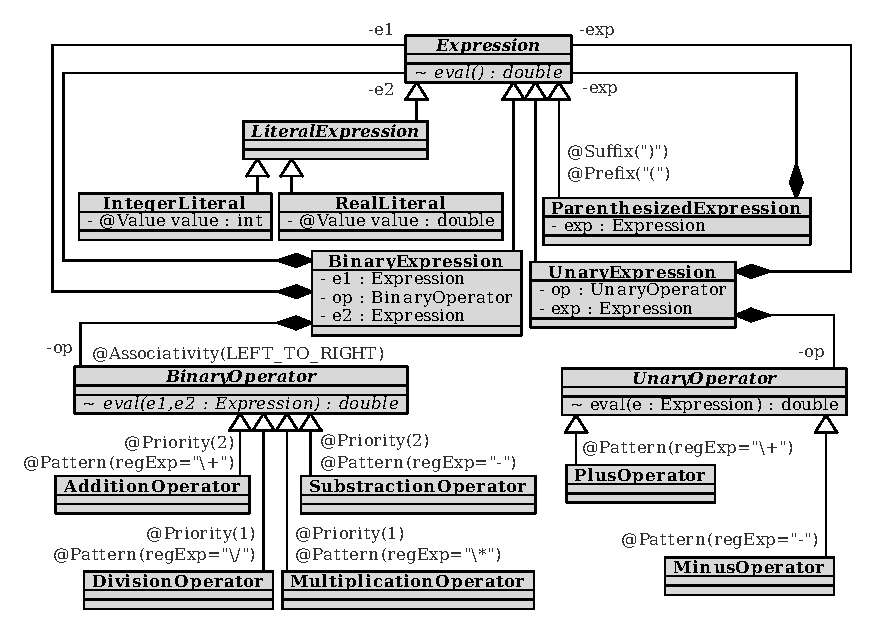
\includegraphics[width=1.00\textwidth]{calculator2.eps}\\[-1.5cm]

\subsubsection{Java class implementation}
The full functional implementation of this example (including valid import and package statements) can be found in the ModelCCExamples library, which is included in the source and binary distribution packages in the download section of the site (www.modelcc.org).

\begin{colframe}
\begin{verbatim}
public abstract class Expression implements IModel {
  public abstract double eval();
}

@Prefix("\\(") @Suffix("\\)")
public class ParenthesizedExpression
         extends Expression implements IModel {
  Expression e;
  @Override public double eval() {
    return e.eval();
  }
}

public abstract class LiteralExpression
         extends Expression implements IModel {
}

public class UnaryExpression
         extends Expression implements IModel {
  UnaryOperator op;
  Expression e;
  @Override public double eval() {
    return op.eval(e);
  }
}

public class BinaryExpression
         extends Expression implements IModel {
  Expression e1;
  BinaryOperator op;
  Expression e2;
  @Override public double eval() {
    return op.eval(e1,e2);
  }
}

public class IntegerLiteral
         extends LiteralExpression implements IModel {
  @Value int value;
  @Override public double eval() {
    return (double)value;
  }
}
\end{verbatim}
\end{colframe}

\begin{colframe}
\begin{verbatim}
public class RealLiteral
         extends LiteralExpression implements IModel {
  @Value double value;
  @Override public double eval() {
    return value;
  }
}

public abstract class UnaryOperator
         implements IModel {
  public abstract double eval(Expression e);
}

@Pattern(regExp="\\+")
public class PlusOperator
         extends UnaryOperator implements IModel {
  @Override public double eval(Expression e) {
    return e.eval();
  }
}

@Pattern(regExp="-")
public class MinusOperator
         extends UnaryOperator implements IModel {
  @Override public double eval(Expression e) {
    return -e.eval();
  }
}

@Associativity(AssociativityType.LEFT_TO_RIGHT)
public abstract class BinaryOperator
         implements IModel {
  public abstract double eval(Expression e1,Expression e2);
}

@Priority(value=2) @Pattern(regExp="\\+")
public class AdditionOperator
         extends BinaryOperator implements IModel {
  @Override public double eval(Expression e1,Expression e2) {
    return e1.eval()+e2.eval();
  }
}
\end{verbatim}
\end{colframe}

\begin{colframe}
\begin{verbatim}
@Priority(value=2) @Pattern(regExp="-")
public class SubstractionOperator
         extends BinaryOperator implements IModel {
  @Override public double eval(Expression e1,Expression e2) {
    return e1.eval()-e2.eval();
  }
}

@Priority(value=1) @Pattern(regExp="\\*")
public class MultiplicationOperator
         extends BinaryOperator implements IModel {
  @Override public double eval(Expression e1,Expression e2) {
    return e1.eval()*e2.eval();
  }
}

@Priority(value=1) @Pattern(regExp="\\/")
public class DivisionOperator
         extends BinaryOperator implements IModel {
  @Override public double eval(Expression e1,Expression e2) {
    return e1.eval()/e2.eval();
  }
}
\end{verbatim}
\end{colframe}

\subsection{Canvas Draw language} \label{sec:langcanv}

The Canvas Draw language allows the imperative generation of drawings.

\subsubsection{Language Specification}

The Canvas Draw language features the following capabilities:

\begin{itemize}
\item Setting the canvas width, height, and background color.
\item Changing the current color.
\item Changing the current stroke width.
\item Drawing lines, rectangles, circles, ovals, polygons, filled rectangles, filled circles, filled ovals, and filled polygons.
\item Each of the elements is described in a particular way (list of coordinates, coordinates and radius, ...).
\end{itemize}

Example input and output:
\begin{itemize}
\item Input:
\begin{verbatim}
   canvas                                 % Creates a canvas
        width 640                         % with width 640,
        height 480                        % height 480,
        background (92,164,169)           % and a cyan background.
                                          % Then:
      color (31,41,56)                    % Sets the color to dark cyan
      stroke 5                            % Sets the stroke to 5
      line [(10,10),(40,40)]              % Draws a line at (10,10) to (40,40)
      rectangle [(40,100),(60,120)]       % Draws a rectangle at (40,100) to (60,120)
      circle (400,30),400      
\end{verbatim}
\begin{itemize} \item Output: \\
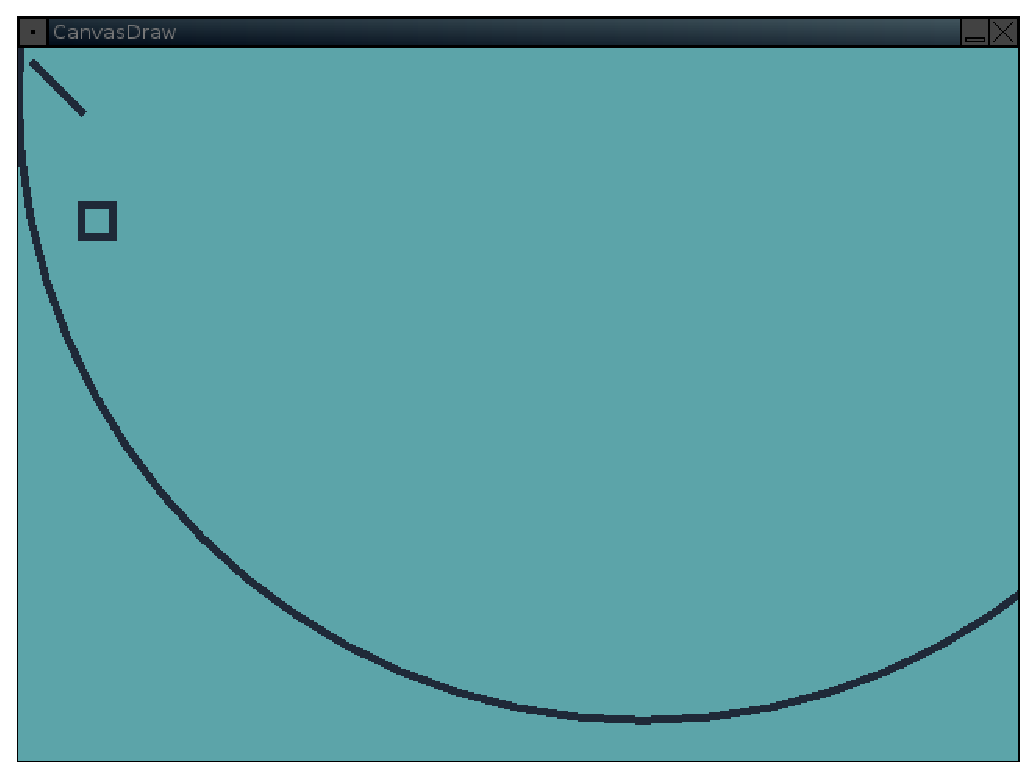
\includegraphics[width=0.70\textwidth]{canvas1.eps}
\end{itemize}

\item Input:
\begin{verbatim}
   canvas                                 % Creates a canvas
        width 800                         % with width 800,
        height 600                        % height 600,
        background (0,0,0)                % and a black background.
                                          % Then:
      color (180,40,40)                   % Sets the color to red
      rectangle [(40,100),(60,120)] fill  % Draws a fill rectangle at (40,100) to (60,120)
      oval [(300,200),(400,370)] fill     % Draws an oval at (300,200) to (400,370)
      stroke 3                            % Sets the stroke to 3
      line [(150,150),(200,200)]          % Draws a line at (150,150) to (200,200)
      color (40,180,40)                   % Sets the color to green
      stroke 7                            % Sets the stroke to 7
      circle (400,30),400                 % Draws a circle of radius 400 at (400,30)
      color (70,70,180)                   % Sets the color the purple
      polygon [(120,160),(110,140),       % Draws a fill polygon.
              (165,130),(186,180)] fill
\end{verbatim}
\begin{itemize} \item Output: \\
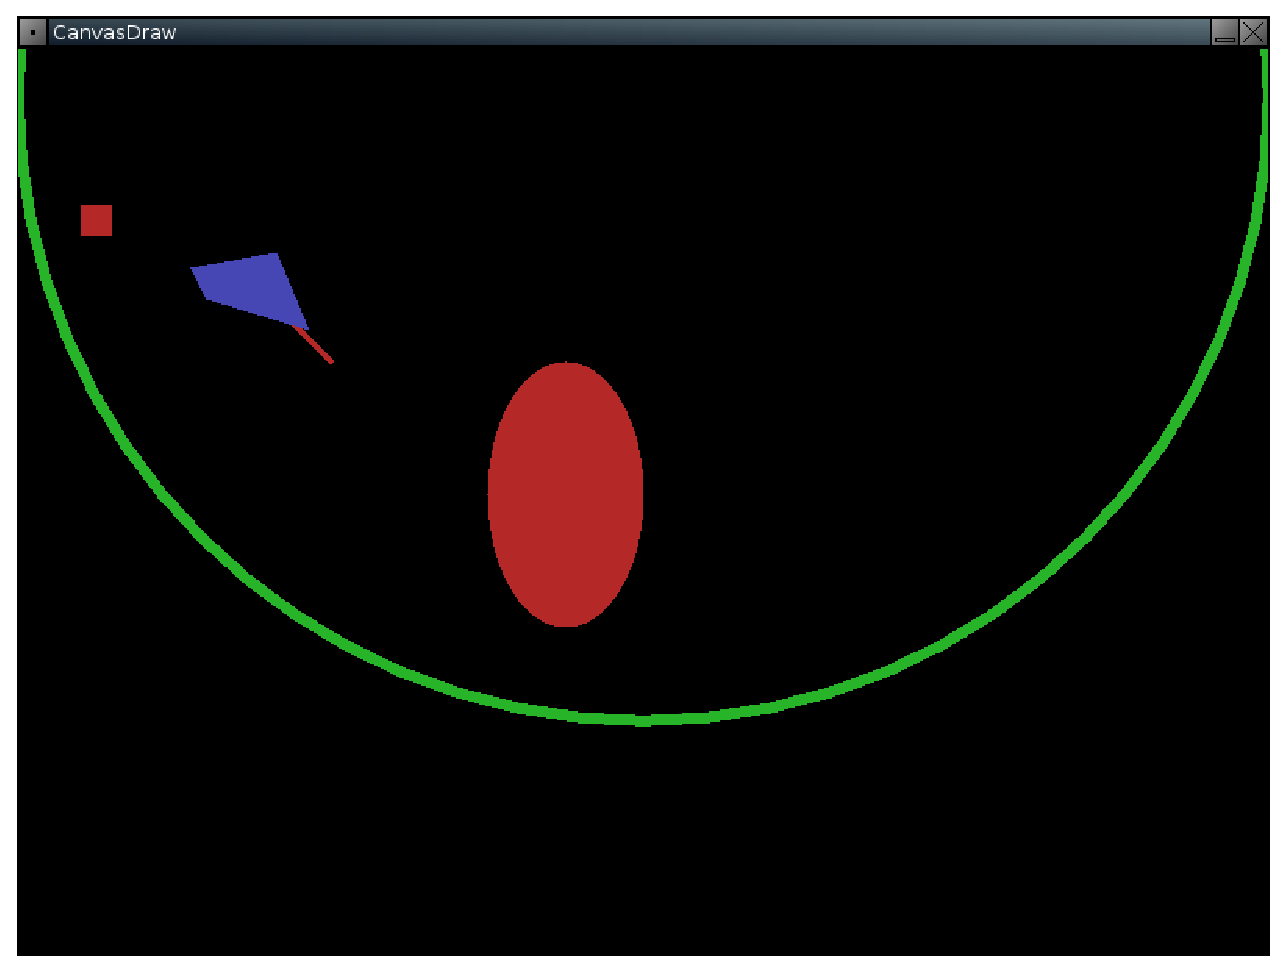
\includegraphics[width=0.80\textwidth]{canvas2.eps}
\end{itemize}
\end{itemize}


\subsection{Imperative Arithmetic language} \label{sec:langimpa}

The Imperative Arithmetic language processes processes assignment and output sentences containing arithmetic expressions in infix notation.

\subsubsection{Language Specification}
The Imperative Arithmetic language features the following capabilities:

\begin{itemize}
\item Unary operators: +, and -.
\item Binary operators: +, -, *, and /, being - and / left-associative.
\item Operator priorities: * and / precede + and -.
\item Parenthesized expressions.
\item Integer and floating-point literals.
\item Binary operators: +, and -.
\item Variables: different references to the same variable are links to the same object.
\end{itemize}

Example input and output:

\begin{itemize}
\item Input:
\begin{verbatim}
variables
  var a
  var b
  var c
sentences
  a = 1
  b = a+2
  c = (a+b)*2
  output a
  output b
  output c
\end{verbatim}
\begin{itemize} \item Output:
\begin{verbatim}
1.0
3.0
8.0
\end{verbatim}
\end{itemize}
\end{itemize}

%\fancyhead[LE]{}
%\newpage
%\bibliographystyle{abbrv}
%\bibliography{doc}
%\fancyhead[LE]{\rightmark}

%\newpage
%\pagestyle{empty}
%\cleardoublepage
%\empt
%\rule{0cm}{10cm}
%\begin{center}
%ModelCC User Guide
%\end{center}
\end{document}
